% ============================================================
%  hw4_statement.tex
%  Re-typesetting of hw4.pdf (MATH 6660, Homework 4, Fall 2026).
%  Statement only -- nothing added, nothing removed, nothing corrected.
%  Text transcribed from hw4.pdf; page geometry not measured (unlike HW3).
%  The element sketch in 4(c) is drawn with TikZ instead of the embedded image.
%  Build:  pdflatex hw4_statement.tex
% ============================================================
\documentclass[11pt]{article}

\usepackage[letterpaper,left=40.9pt,right=61pt,top=77.2pt,bottom=90pt,
            headheight=30pt,headsep=15.6pt,footskip=28.3pt]{geometry}
\usepackage[T1]{fontenc}
\usepackage{amsmath,amssymb}
\usepackage{enumitem}
\usepackage{fancyhdr}
\usepackage{tikz}
\usepackage{hyperref}

\pagestyle{fancy}
\fancyhf{}
\fancyhead[R]{\textbf{Assigned:} Monday Oct. 26, 2026\\
              \textbf{Due:} Monday Nov. 9, 2026}
\fancyfoot[C]{\thepage}
\renewcommand{\headrulewidth}{0.4pt}

\setlength{\parindent}{0pt}
\setlist[enumerate,1]{leftmargin=27.1pt,labelsep=5.5pt,topsep=9pt,itemsep=9pt,parsep=0pt}
\setlist[enumerate,2]{label=(\alph*),leftmargin=24pt,labelsep=5.5pt,topsep=6pt,itemsep=6pt,parsep=0pt}

% section heading: bold, underlined (as in hw4.pdf)
\newcommand{\hwsection}[1]{\par\vspace{2pt}\noindent{\Large\bfseries\underline{#1}}\par\vspace{3pt}}
\newcommand{\cln}{\;{:}\quad}

\begin{document}

\begin{center}
  {\large\textsc{MATH 6660: Homework 4}}\\
  {\large\textsc{Fall 2026}}
\end{center}

\hwsection{2D Unstructured FEM:}

\begin{enumerate}

\item Download the PyDistMesh mesh generator. You can find all the necessary
links from the Math 6660 Canvas page.

\item Use this code to generate a mesh for the following geometry: a
star-shaped region. The boundary of this region is the zero contour of the
following function:
\[
  \phi(r,\theta) = r - 0.75 - 0.25\sin(5\theta).
\]

\item Use the CG(1) method developed in class and provided in the Math 6660
Canvas page to solve the following Poisson equation on the star-shaped domain
created in Problem \#2:
\begin{align*}
  \textbf{PDE} &\cln -u_{,x,x} - u_{,y,y} = 1 \quad\text{in}\quad \Omega,\\
  \textbf{BCs} &\cln u = 0 \quad\text{on}\quad \partial\Omega.
\end{align*}

\end{enumerate}

\hwsection{2D Cartesian FEM:}

\begin{enumerate}[resume]

\item Consider the 2D Poisson equation:
\begin{align*}
  \textbf{PDE} &\cln -\nabla\cdot\nabla u = f(x,y) \quad\text{in}\quad
                 \Omega = [-1,1]\times[-1,1]\,,\\
  \textbf{BC}  &\cln u = g \quad\text{on}\quad \partial\Omega.
\end{align*}

\begin{enumerate}

\item Recast this problem as a variational problem. Clearly state the test and
trial function spaces.

\item Show that the variational problem has a unique solution by showing that
it meets all of the criteria of the Lax-Milgram theorem.

\item Develop a finite element method for this problem based on square (not
triangular) elements of the form:
\begin{center}
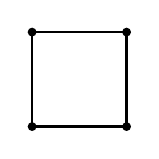
\begin{tikzpicture}[scale=1.0]
  \draw[thick] (0,0) rectangle (1.2,1.2);
  \foreach \p in {(0,0),(1.2,0),(0,1.2),(1.2,1.2)} \fill \p circle (1.6pt);
\end{tikzpicture}
\end{center}
On each element, the solution on the four corners is interpolated with the
following interpolant:
\[
  s(x,y) = \alpha_1 + \alpha_2 x + \alpha_3 y + \alpha_4 xy.
\]
Write out the basis functions and explicitly write out the linear system that
arises from your FEM (you can just assume that the grid spacing in $x$ and $y$
are the same and uniform).

\item Use this method to solve the 2D Poisson equation with
\begin{align*}
  f(x,y) &= \pi^{2} e^{\sin(\pi x)\sin(\pi y)}
    \left\{2\sin(\pi x)\sin(\pi y) + 2\cos^{2}(\pi x)\cos^{2}(\pi y)
    - \cos^{2}(\pi x) - \cos^{2}(\pi y)\right\},\\
  g(x,y) &= 1.
\end{align*}
Create a convergence table showing both $\|\cdot\|_{V}$ and
$\|\cdot\|_{L^{2}(\Omega)}$ errors. What order of convergence do you observe?
In this case the exact solution is
\[
  u(x,y) = e^{\sin(\pi x)\sin(\pi y)}.
\]

\end{enumerate}

\end{enumerate}

\end{document}
